\documentclass[12pt, journal, onecolumn]{IEEEtran}
\raggedbottom
%
\usepackage{instructivo}  % Commands for multiple choice
\graphicspath{{./}{./fig/}}

\usepackage[natbib=true,style=trad-unsrt,backend=biber]{biblatex}

\addbibresource{literatura.bib}
\usepackage{multirow}
\usepackage{graphicx}
\usepackage{array}
\usepackage{float}
\usepackage{capt-of}
\usepackage{hyperref}
\newcolumntype{C}{>{\centering\arraybackslash}X}
% correct bad hyphenation here
\hyphenation{op-tical net-works semi-conduc-tor}


\begin{document}
	%
	% paper title
	% Titles are generally capitalized except for words such as a, an, and, as,
	% at, but, by, for, in, nor, of, on, or, the, to and up, which are usually
	% not capitalized unless they are the first or last word of the title.
	% Linebreaks \\ can be used within to get better formatting as desired.
	% Do not put math or special symbols in the title.
\title{Proyecto: Semáforo Vehicular y Peatonal}
	
	
\author{Gerald~David~Blanco-Sáenz,~\IEEEmembership{Estudiante,~ITCR},~Melanie~Espinoza-Hernandez,~\IEEEmembership{Estudiante,~ITCR},~Nayshell~Freckleton-White,~\IEEEmembership{Estudiante,~ITCR} 
	y~Pablo~Cabrera-Montealegre,~\IEEEmembership{Estudiante,~ITCR}}
	
	
	% The paper headers
\markboth{EL3215 Laboratorio de Electrónica Analógica, IS2026}%
{EL3215 Laboratorio de Electrónica Analógica}
	
	
	% make the title area
\maketitle
	
\begin{abstract}
		Se propone el diseño de un sistema de semáforo vehicular y peatonal, cuyo objetivo principal es simular un cruce vehicular completo mediante la gestión del flujo de tránsito y la interacción a través de solicitudes peatonales. El sistema incorpora señalización visual (rojo, amarillo, verde) y auditiva, control de tiempos regresivos mediante displays, y una etapa de conversión de energía de corriente alterna (CA) a corriente directa (CD). En este primer avance, se documenta exclusivamente la etapa de alimentación del circuito, la cual es responsable de proveer los niveles de tensión regulados adecuados para el funcionamiento de las etapas analógicas y digitales posteriores.
\end{abstract}
	
\section{Introducción}
	Los sistemas de control de tráfico son fundamentales para la regulación segura y eficiente de la movilidad vehicular y peatonal en entornos urbanos. Estos sistemas integran elementos de temporización, señalización visual y auditiva, así como mecanismos de interacción con los usuarios. En el contexto de la ingeniería electrónica, el diseño de un sistema de semáforo permite aplicar conceptos relacionados con la generación de señales, temporización, control lógico, visualización de información y procesamiento de señales de audio. Además, representa un ejemplo claro de integración de subsistemas analógicos y digitales en una aplicación real. \\
	
	Este proyecto se enfoca en el diseño e implementación de un sistema completo de semáforo vehicular y peatonal, utilizando componentes electrónicos discretos y circuitos digitales básicos, evitando el uso de dispositivos programables de acuerdo con las especificaciones. El objetivo principal de este primer documento es presentar la propuesta de diseño de cada etapa del sistema, detallando sus componentes y la justificación de las decisiones de diseño.
	
	\section{Objetivos}
	\subsection{Objetivo General}
	Introducir al estudiante ante un problema de ingeniería en donde requiera poner en práctica las habilidades y conceptos adquiridos en el uso de las herramientas de simulación, equipos de medición, prototipado y ensamble de circuitos eléctricos transistorizados por medio de circuitos impresos.
	
	\subsection{Objetivos Específicos}
	\begin{itemize}
		\item Introducir al estudiante en el diseño de ingeniería bajo el establecimiento de una solución a un problema planteado.
		\item Utilizar herramientas de simulación en la etapa de diseño de sistemas electrónicos que integren etapas analógicas y digitales.
		\item Desarrollar habilidades de implementación de sistemas electrónicos bajo el apoyo de equipo especializado para mediciones.
		\item Adquirir conocimiento y habilidades necesarias para el diseño e implementación de circuitos impresos o PCB para ensamble de circuitos eléctricos.
		\item Fomentar las habilidades requeridas para el trabajo en equipo en proyectos de ingeniería.
	\end{itemize}
	
	\section{\textbf{Alimentación}}
	\subsection{Descripción}
	Para el funcionamiento del semáforo eléctrico y sus respectivos sistemas lógicos, se requiere una fuente de alimentación que convierta la energía proveniente de la red eléctrica de 120\,$\text{V}_{\text{rms}}$ a 60\,Hz en niveles de tensión de corriente directa (CD) regulados y ajustados. Estos voltajes son vitales para cumplir con las condiciones de operación de las compuertas lógicas, los circuitos de temporización y las etapas de potencia para la señalización visual y acústica.\\
	
	El circuito convertidor de CA a CD incluye los siguientes componentes principales: un transformador reductor, un puente rectificador de onda completa, capacitores de filtrado y reguladores de voltaje lineal. Estos elementos actúan en conjunto para entregar las tensiones estables que requiere el resto del sistema, protegiendo los componentes de variaciones indeseadas.
	
	\subsection{Diagrama del circuito}
	% Descomente y ajuste el nombre de la imagen:
	\begin{figure}[h]
		\centering
		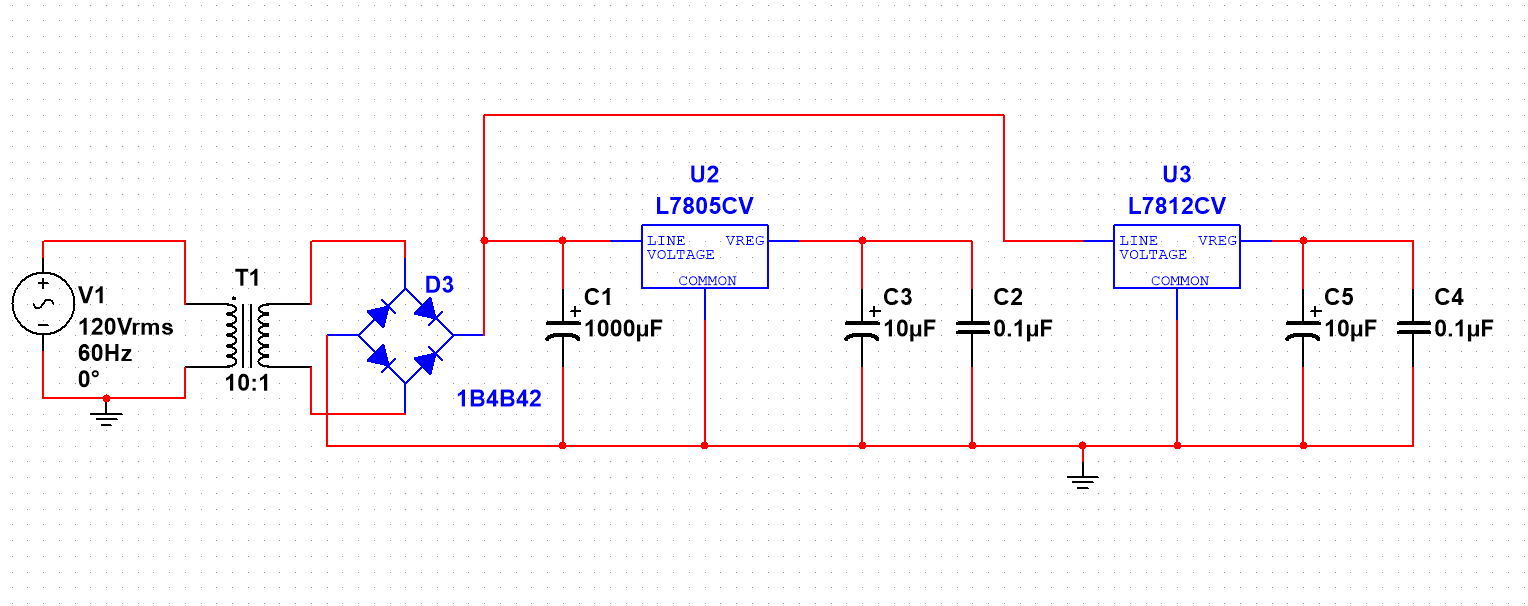
\includegraphics[width=0.7\textwidth]{diagrama_alimentacion.png}
		\caption{Diagrama del circuito de Alimentación.}
		\label{fig:alimentacion}
	\end{figure}
	
	\subsection{Justificación de diseño}
	El diseño del circuito de alimentación de la Fig. \ref{fig:alimentacion} se fundamenta en la necesidad de convertir los 120\,$\text{V}_{\text{rms}}$ de corriente alterna (CA) a voltajes de corriente directa (CD) regulados estables, habitualmente de 5\,V para los componentes de lógica digital (TTL/CMOS), y otros voltajes mayores (como 12\,V) si así lo requieren la amplificación de la señal acústica o los arreglos de LEDs de alta luminosidad.\\
	
	Inicialmente, el transformador reductor disminuye el voltaje de entrada a un nivel seguro y apto para su manipulación. Luego, el puente rectificador de diodos convierte la señal alterna en una señal pulsante en una sola dirección. Para disminuir el rizado de esta señal, se incorporan capacitores de gran valor en capacitancia que filtran las oscilaciones y otorgan una primera etapa de estabilización a la señal.\\
	
	Finalmente, los reguladores de voltaje integrados (como los de la familia 78XX) proporcionan una salida continua y fija, absorbiendo las variaciones en el consumo de corriente al encender diferentes estados del semáforo. Se agregan capacitores de desacople adicionales en los terminales de entrada y salida de estos reguladores para estabilizar la respuesta transitoria del dispositivo y atenuar posibles ruidos de alta frecuencia introducidos por la conmutación lógica, garantizando así un desempeño ininterrumpido en todo el circuito de control de tráfico.\\

\newpage

\section{\textbf{Máquina de estados}}
\subsection{Descripción}
Esta subsección describe el circuito encargado de controlar la lógica completa del semáforo vehicular y peatonal, incluyendo la generación de estados, temporización, control de transición y activación de las señales luminosas. El circuito implementa una máquina de estados síncrona basada en lógica digital discreta, utilizando compuertas lógicas, contadores y temporizadores, cumpliendo con las especificaciones establecidas para el proyecto de semáforo vehicular y peatonal.\\

Para facilitar el análisis del sistema, el circuito se divide en cuatro bloques funcionales principales: el generador de reloj, la máquina de estados principal, la lógica de decodificación y control, y la etapa de señalización visual del semáforo.\\

El generador de reloj se implementa mediante un 555 configurado en modo astable, el cual produce una señal cuadrada periódica utilizada como señal de sincronización del sistema.\\

La máquina de estados principal se implementa utilizando un contador CD4017BP, el cual activa secuencialmente sus salidas $Q_0$ a $Q_9$ con cada flanco positivo de reloj. Cada salida representa un estado específico del sistema de semáforo. La secuencia inicia en $Q_0$, donde el semáforo vehicular permanece en verde y el peatonal en rojo hasta que el usuario presione el botón peatonal. Una vez recibido el pulso del botón, el sistema comienza la secuencia automática de transición.\\

Las señales provenientes de las salidas del CD4017BP son procesadas mediante compuertas lógicas 74LS08 (AND), 74LS32 (OR) y 74LS14 (Schmitt Trigger Inverter). Estas compuertas permiten combinar múltiples estados para generar correctamente las señales de control de los LEDs vehiculares y peatonales. Además, la compuerta Schmitt Trigger se utiliza para limpiar y estabilizar las transiciones provenientes del contador y evitar problemas asociados al ruido o a señales intermedias.\\

La etapa de señalización visual está conformada por LEDs indicadores correspondientes al semáforo vehicular y peatonal. Cada LED cuenta con una resistencia limitadora para proteger los dispositivos ante sobrecorriente. El semáforo vehicular utiliza LEDs rojo, amarillo y verde, mientras que el sistema peatonal utiliza LEDs rojo y verde. La activación de cada LED depende directamente de la lógica generada por las compuertas asociadas a los distintos estados de la máquina.\\

El funcionamiento general del sistema consiste en mantener el semáforo vehicular en verde hasta recibir una solicitud peatonal. Posteriormente, el sistema realiza una secuencia de parpadeo del verde vehicular, cambia a amarillo durante un intervalo fijo y finalmente habilita el paso peatonal mediante el LED verde peatonal y el LED rojo vehicular. Finalizada la secuencia, el contador se reinicia automáticamente y el sistema vuelve al estado inicial.
 \\

\subsection{Diagrama del circuito}
	% Descomente y ajuste el nombre de la imagen:
	
	\begin{figure}[H]
		\centering
		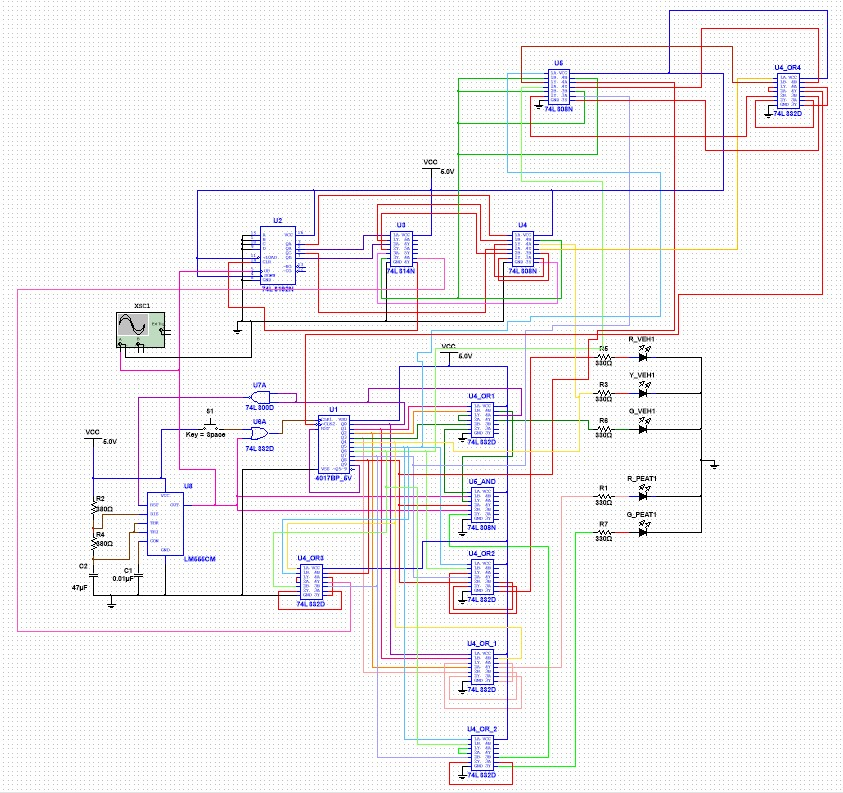
\includegraphics[width=0.7\textwidth]{Diagrama_Multisim_FSM.jpg}
		\caption{Diagrama del circuito de la FSM con los leds en el software Multisim.}
		\label{fsm1}
	\end{figure}
	
	
	
\subsection{Justificación de diseño}

\subsubsection{\textbf{Generador de reloj}}
El generador de reloj se implementó utilizando el LM555CM en configuración astable debido a su simplicidad, estabilidad y facilidad para ajustar la frecuencia mediante componentes pasivos externos. Este circuito permite generar una señal cuadrada compatible con niveles TTL de 5 $V$, adecuada para excitar directamente el CD4017BP y el resto de la lógica digital.\\

La frecuencia del reloj se ajustó aproximadamente a 1 Hz para que cada transición de estado representara un segundo real, simplificando así la implementación de los tiempos requeridos para el semáforo. El capacitor conectado al pin de control del LM555CM se incorporó para filtrar ruido y mejorar la estabilidad temporal del sistema.\\

\subsubsection{\textbf{Máquina de estados principal}}
La máquina de estados principal se diseñó utilizando un CD4017BP debido a que este dispositivo permite generar una secuencia ordenada de estados sin necesidad de memorias adicionales o lógica secuencial compleja. Cada salida del contador representa directamente un estado específico del sistema, simplificando considerablemente la implementación física del semáforo.\\

La asignación de estados se realizó de la siguiente manera:

\begin{itemize}
    \item $Q_0$: semáforo vehicular en verde fijo y peatonal en rojo. Este estado permanece activo indefinidamente hasta recibir una solicitud peatonal.
    
    \item $Q_1$, $Q_2$ y $Q_3$: corresponden al parpadeo del LED verde vehicular antes de realizar la transición a amarillo.
    
    \item $Q_4$: activa el LED amarillo vehicular durante aproximadamente 5 segundos.
    
    \item $Q_5$, $Q_6$, $Q_7$ y $Q_8$: corresponden al estado peatonal habilitado, donde el semáforo vehicular permanece en rojo y el peatonal en verde, incluyendo el parpadeo final del LED peatonal.
    
    \item $Q_9$: se utiliza para reiniciar automáticamente el CD4017BP mediante el pin RESET, retornando el sistema al estado inicial.
\end{itemize}

Adicionalmente, el sistema incorpora un módulo de conteo regresivo sincronizado con la máquina de estados, permitiendo controlar la duración exacta de determinados estados del semáforo.\\

El contador inicia automáticamente cuando la máquina entra al estado peatonal y comienza una secuencia regresiva desde 20 hasta 00. La señal de reloj utilizada por los contadores proviene del mismo generador de reloj de 1 Hz empleado en la FSM, garantizando sincronización temporal entre ambos sistemas.\

La transición entre estados depende directamente de la finalización de ciertos intervalos de tiempo. Por ejemplo, el estado amarillo permanece activo durante aproximadamente 5 segundos, mientras que el estado peatonal utiliza el conteo regresivo para determinar el tiempo restante antes del retorno al estado inicial. 

	\begin{figure}[H]
		\centering
		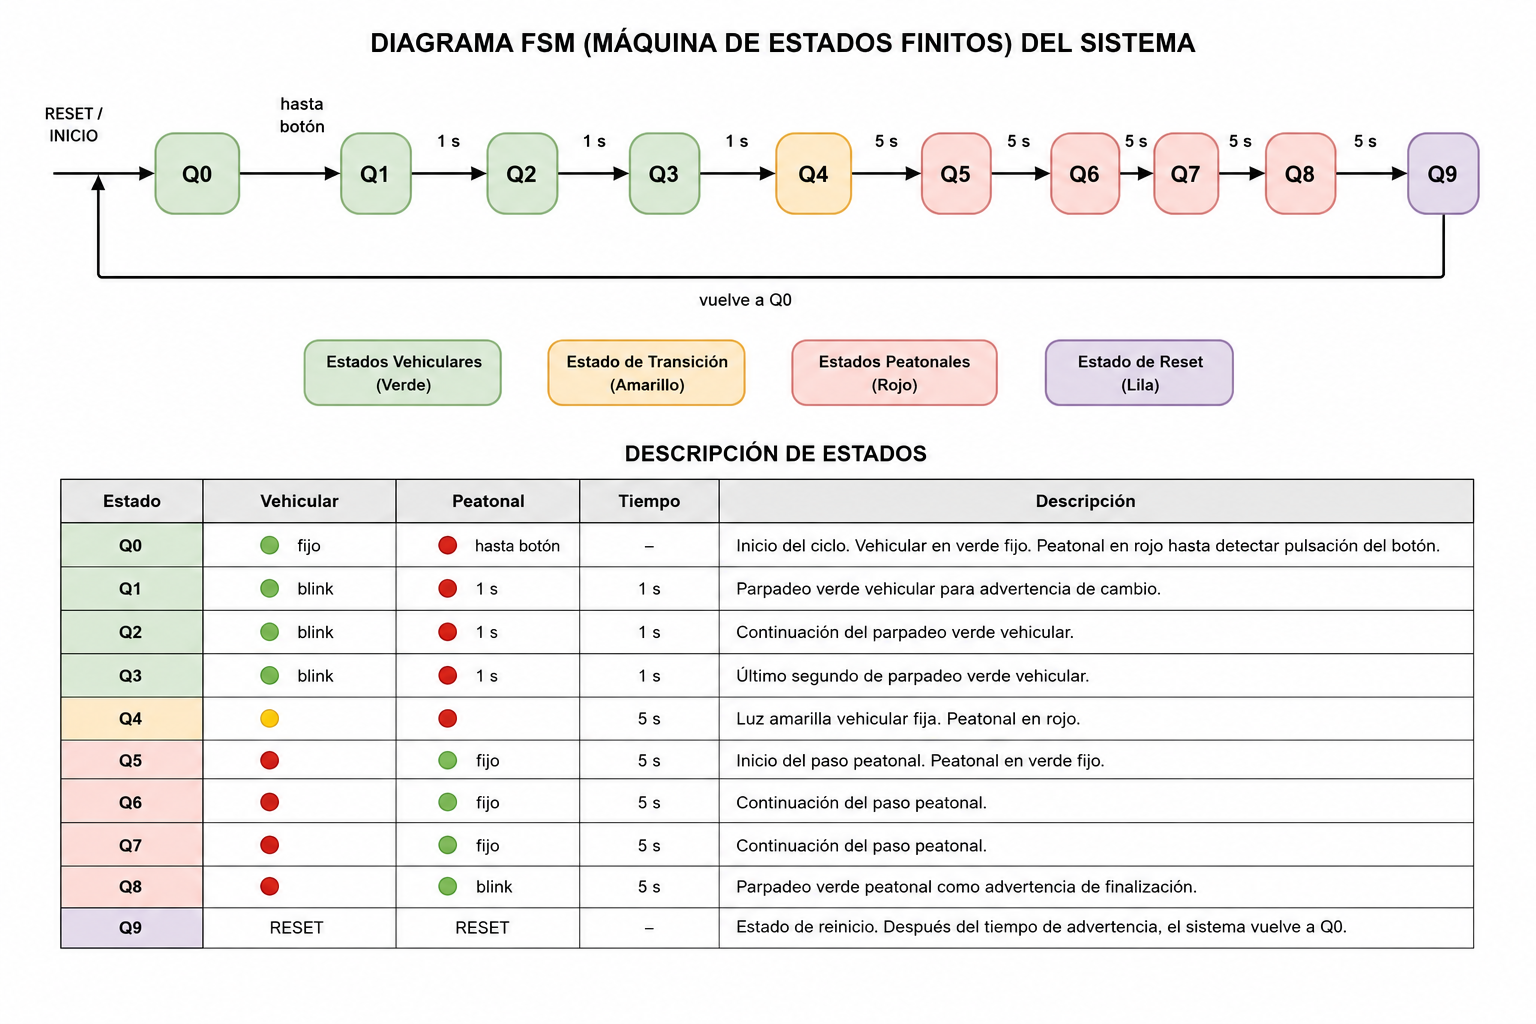
\includegraphics[width=1\textwidth]{Diagrama_de_FSM.png}
		\caption{Diagrama del flujo de la máquina de estado.}
		\label{fsm1}
	\end{figure}

\newpage

\subsubsection{\textbf{Lógica de decodificación}}
La lógica de decodificación se implementó mediante compuertas AND y OR debido a la necesidad de combinar múltiples estados del contador para generar las señales finales de control.\\

Las compuertas 74LS32 y 74LS08 se utilizan para detectar combinaciones específicas de estados y habilitar determinadas transiciones o salidas. Por otro lado, las compuertas 74LS32 permiten unir varios estados del CD4017BP en una sola línea lógica para controlar un mismo LED durante múltiples intervalos de tiempo.\\


\subsubsection{\textbf{Etapa de señalización visual}}
La etapa visual se diseñó utilizando LEDs independientes para cada luz del semáforo vehicular y peatonal, permitiendo una representación clara del estado actual del sistema.\\

Cada LED posee una resistencia limitadora de 330 $\Omega$, seleccionada para mantener una corriente segura de operación y evitar daños en los dispositivos. Esta configuración también garantiza un brillo uniforme y adecuado para visualización durante las pruebas del sistema.\\

El uso de lógica discreta para controlar directamente los LEDs permite observar claramente la transición entre estados y facilita tanto la simulación como el diagnóstico del circuito durante la etapa de implementación física.

\newpage

\section{\textbf{Display 7-Segmentos}}
\subsection{Descripción}
El módulo de display fue diseñado para implementar el conteo regresivo visual del sistema de semáforo vehicular y peatonal. Su función principal consiste en mostrar al usuario el tiempo restante disponible durante la habilitación del paso peatonal.\\

El sistema utiliza un temporizador 555 en configuración astable como generador de pulsos de reloj, encargado de producir la señal periódica que sincroniza el conteo. Esta señal es enviada a dos contadores BCD CD4510, uno destinado al manejo de las unidades y otro al de las decenas del conteo regresivo.\\

Las salidas BCD de cada contador son conectadas a decodificadores CD4511, los Las salidas BCD de cada contador son conectadas a decodificadores CD4511, los cuales convierten la información binaria en las señales necesarias para controlar los displays de 7 segmentos. Además, cada segmento incorpora una resistencia limitadora de corriente de 330\,$\Omega$ con el objetivo de proteger tanto los displays como los circuitos integrados.\\

El módulo fue configurado para iniciar el conteo en 20 segundos, disminuyendo progresivamente hasta llegar a 00, permitiendo visualizar el tiempo restante para el cruce peatonal. Además, se implementará una lógica de detección de cero mediante compuertas lógicas, de manera que cuando el sistema detecta simultáneamente 00 en decenas y unidades, el reloj queda bloqueado y el contador deja de disminuir, evitando conteos inválidos posteriores al cero.


\subsection{Diagrama del circuito}
	% Descomente y ajuste el nombre de la imagen:
	
	\begin{figure}[H]
		\centering
		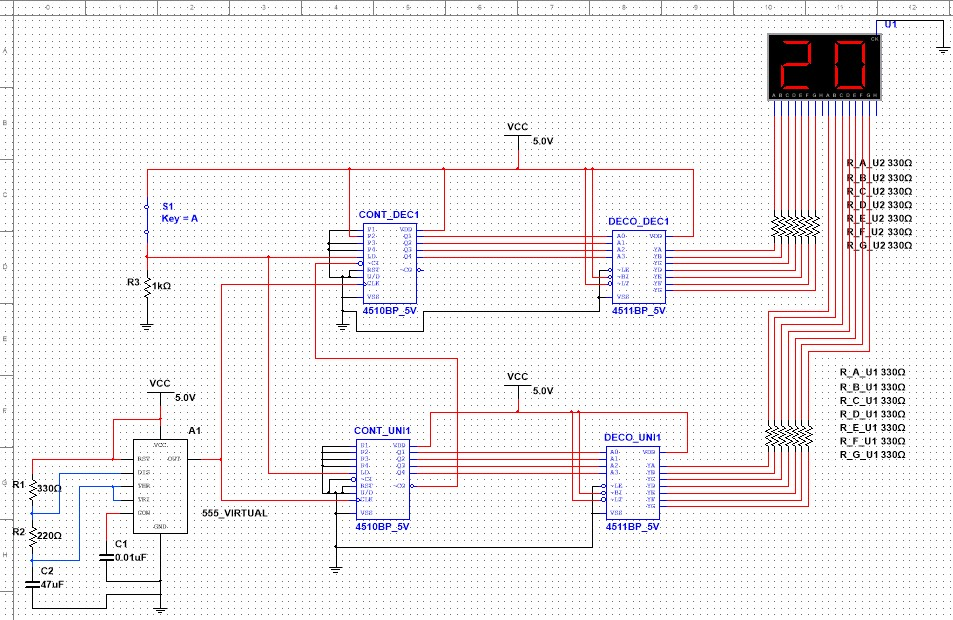
\includegraphics[width=0.9\textwidth]{Diagrama_Multisim_Display.jpg}
		\caption{Diagrama del circuito del Display de 7-segmentos en el software Multisim.}
		\label{diag_circuito_display}
	\end{figure}
		
	
\subsection{Justificación de diseño}
El diseño del módulo de display se desarrolló utilizando componentes digitales discretos debido a la necesidad de implementar un sistema de conteo regresivo confiable, visible y compatible con la lógica general del semáforo peatonal. Se seleccionaron contadores BCD CD4510 porque permiten realizar conteos descendentes de manera sencilla y facilitan la manipulación de valores decimales sin requerir lógica adicional compleja.\\

Asimismo, se emplearon decodificadores CD4511 debido a su compatibilidad directa con displays de 7 segmentos de cátodo común, reduciendo significativamente la cantidad de conexiones y simplificando la implementación física del sistema. Esto permite obtener una visualización clara del tiempo restante para el cruce peatonal.\\

La utilización del temporizador 555 como generador de reloj se debe a su facilidad de configuración, estabilidad y bajo costo, permitiendo generar pulsos periódicos necesarios para sincronizar el conteo del sistema. Además, las resistencias limitadoras fueron incorporadas para proteger los segmentos LED de sobrecorrientes y aumentar la confiabilidad del circuito.\\

Finalmente, de esta manera se puede verificar individualmente que este bloque sea funcional antes de integrar el sistema completo del semáforo.\\


\begin{figure}[H]
		\centering
		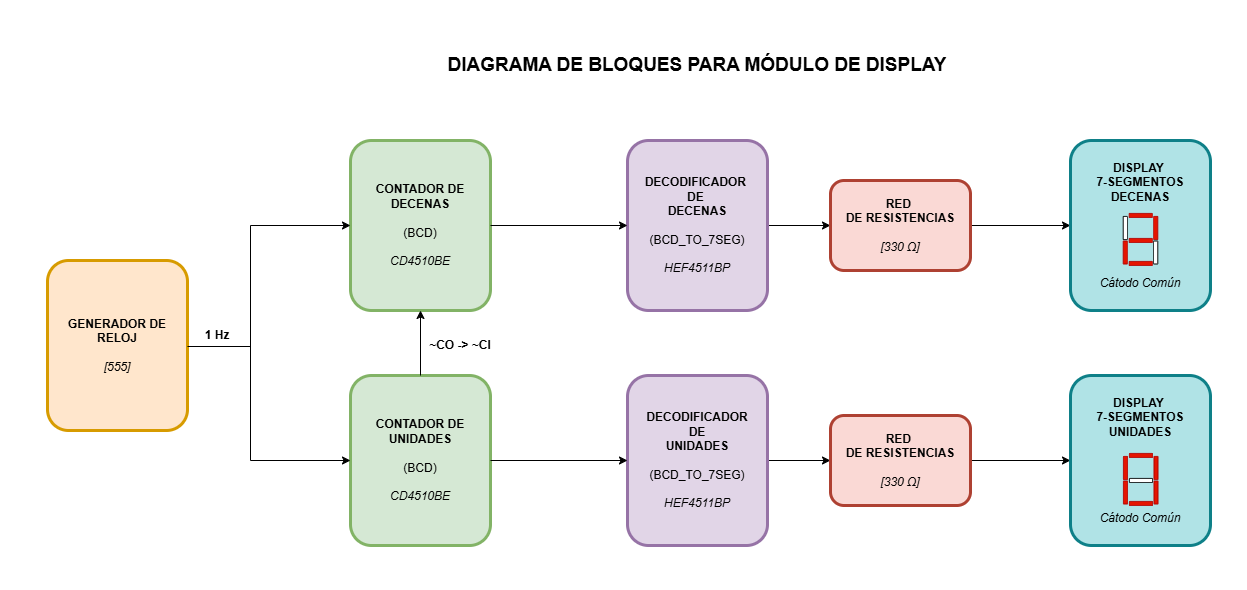
\includegraphics[width=1\textwidth]{Diagrama_de_bloques_Display.png}
		\caption{Diagrama de bloques para el Display.}
		\label{diag_bloq_display}
	\end{figure}
	
\newpage
	
\section{\textbf{Sistema de Señalización Auditiva}}

\subsection{Descripción}
Este sistema fue diseñado con el propósito de generar una señal auditiva para los peatones cuando este permitido cruzar la calle. Consiste en generar un sonido periódico cuando el semáforo peatonal se encuentre en verde y que este mismo se acelera una vez que falten cinco segundos para que se vuelva a poner en rojo. \\

Tomando en cuenta las especificaciones solicitadas cumpliendo únicamente con el uso de electrónica básica y sin ningún tipo de microcontroladores, se llego a la conclusión que la mejor forma de manejarlo era por medio de osciladores RC con la que se pueden ajustar la frecuencias y compuertas Schmitt Trigger acompañadas de un amplificador para el sonido de salida.\\

Dado estos requerimientos se pude decir que el sistema completo se divide en cuatro bloques funcionales principales:
\begin{enumerate}
    \item Generación del tono audible.
    \item Generación de la frecuencia de repetición lenta.
    \item Generación de la frecuencia de repetición rápida.
    \item Etapa de selección y amplificación de potencia.
\end{enumerate}

En cuanto al funcionamiento del circuito, todo empieza generando una señal de una frecuencia audible (en este caso unos 2kHz aproximadamente) por medio de un oscilador principal. Se selecciona esta frecuencia ya que se encuentra dentro del rango perceptible por el oído humano siendo perceptible fácilmente.
Adicional a esto, se generan además dos osciladores mas de aproximadamente 1Hz y 5Hz sujetos a modificaciones según las pruebas del circuito ensamblado en físico.\\

Estas señales no funcionan como audio directamente, sino que al combinarse lógicamente generan periodos de activación de la señal de tono según la velocidad que sea deseada y dependiendo directamente del estado del semáforo peatonal.\\

Dependiendo del estado en el que se encuentre el semáforo y ligado a la parte de la maquina de estados se generan posteriormente dos compuertas AND con las que se selecciona la velocidad del tono que se desea en cierto momento admitiendo como entradas para cada una la señal rápida o lenta y una señal que se puede interpretar como los 'últimos 5s'. Mediante esto, solo una de las señales debería estar activa en un momento determinada, pero por medidas de seguridad, se implementa entra las salidas de ambas una compuerta OR con las que se asegura que en ningún momento se activen ambas señales produciendo bugs. A la salida de esta compuerta se adiciona nuevamente un AND para así tener la suma del selector de velocidad y el tono audible y que se esta manera suene la bocina cuando la señal de velocidad deseada esta activa.\\

Finalmente, se toma la señal resultante y se pasa por una etapa amplificadora con un transistor NPN en configuración de conmutación ya que no es necesario utilizar un amplificado líneal mas complicado porque se tienen como salida ya una señal cuadrada.\\

\subsection{Diagrama del circuito}

	\begin{figure}[H]
		\centering
		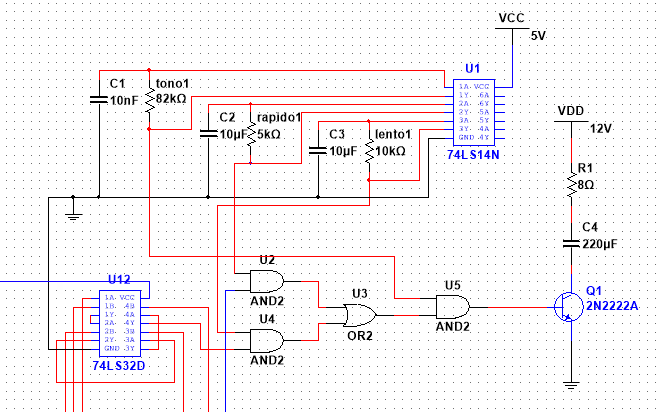
\includegraphics[width=0.7\textwidth]{circ audio.png}
		\caption{Diagrama del circuito de señalización auditiva.}
		\label{audio}
	\end{figure}

\subsection{Justificación de Diseño}
\begin{itemize}
	\item{Compuerta Schmitt Trigger 74LS14}
		Se selecciono un circuito integrado 74LS14 por la necesidad de generar señales cuadradas de un voltaje en corriente continua. Permite se manera sencilla implementar osciladores RC con bastante estabilidad evitando problemas de ruido y transiciones. Ademas, permite la generación de varios osciladores con un mismo circuito conectando una entrada y salida mediante una resistencia y un capacitor entre la entrada y tierra. Esto genera que conforme los valores elegidos de cada componente y según la carga o descarga del capacitor se genere de manera simple una señal cuadrada.\\
		
	\item{Compuertas AND/OR}
		Permiten procesar la lógica necesaria para que no haya bugs en el sistema. Permiten una selección de velocidad de pitidos y una mezcla de estos con la señal audible.\\
		
	\item{Transistor NPN}
		El transistor NPN fue seleccionado debido a que las compuertas lógicas no son capaces de suministrar la corriente necesaria para alimentar directamente el parlante. El transistor añade corriente y por ende potencia entre la lógica digital y logra que la carga de salida sea audible más fácilmente.
		Como beneficio adicional, esta configuración protege las compuertas lógicas contra sobrecorrientes y permite utilizar una fuente de alimentación de mayor voltaje para aumentar el volumen del sonido emitido.\\
		
	\item{Resistencia de Base}
		La resistencia conectada a la base del transistor limita la corriente de entrada, evitando daños tanto en la salida lógica como en el transistor. Este componente resulta fundamental para garantizar una operación segura del sistema.\\
		
	\item{Parlante}
		Se utilizó un parlante de baja impedancia como dispositivo de salida debido a su simplicidad y facilidad de integración. El uso de ondas cuadradas permite generar tonos audibles claramente distinguibles sin necesidad de circuitos de audio complejos.
\end{itemize}

\subsection{Gráficas}

\begin{figure}[H]
    \centering
    \begin{minipage}{0.45\textwidth}
        \centering
        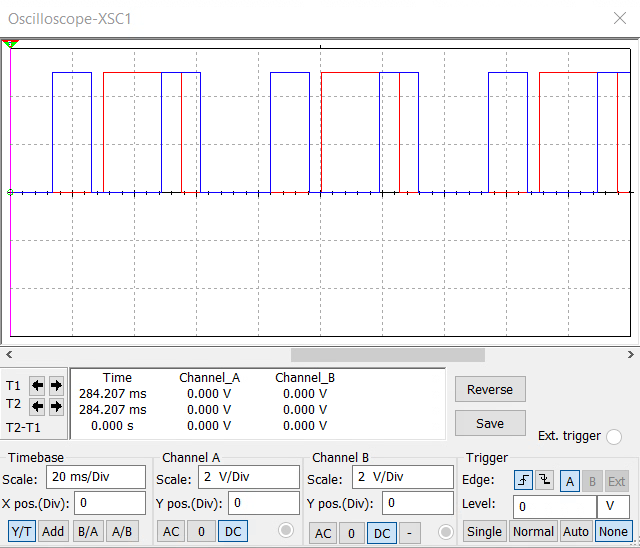
\includegraphics[width=0.9\textwidth]{osc velocidad.png}
		\caption{Señal de oscilación segun seleccion de velocidad.}
    \end{minipage}
    \hfill
    \begin{minipage}{0.45\textwidth}
        \centering
        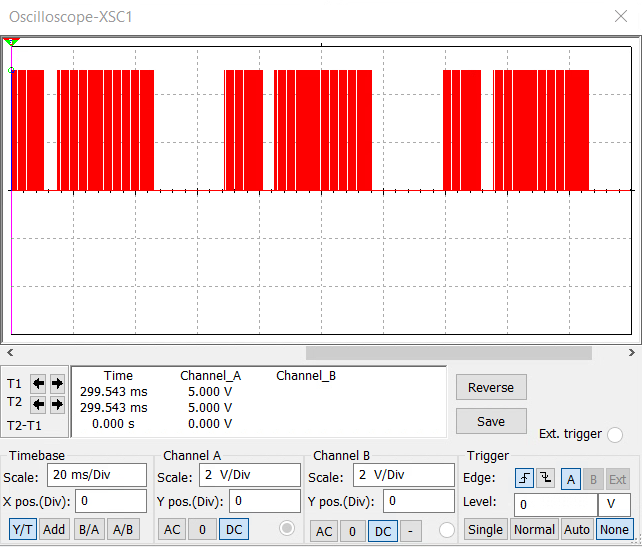
\includegraphics[width=0.9\textwidth]{salida lento.png}
		\caption{Ejemplo de tono de salida en modo lento.}
    \end{minipage}

\end{figure}

\newpage

\begin{thebibliography}{99}

\bibitem{Floyd}
T. L. Floyd, \textit{Dispositivos Electrónicos}, 8.a ed. México: Pearson Prentice Hall, 2008.

\bibitem{555video}
MADE IN COLOMBIA, ``Circuito integrado 555 explicación completa,'' YouTube, Dec. 16, 2017. [Online]. Available: \url{https://www.youtube.com/watch?v=n15R_n_TshA}

\bibitem{555delay}
``Cómo construir un circuito temporizador 555 con un retardo de apagado,'' Learning About Electronics. [Online]. Available: \url{https://www.learningaboutelectronics.com/Articulos/Circuito-temporizador-555-con-retardo-de-apagado.php}

\bibitem{CD4017video}
ElectronicaLED, ``Conexión y funcionamiento del circuito integrado CD4017,'' YouTube, Jun. 27, 2020. [Online]. Available: \url{https://www.youtube.com/watch?v=WflcnppydVY}

\bibitem{4017datasheet}
``IC 4017 Datasheet,'' ElecCircuit. [Online]. Available: \url{https://www.eleccircuit.com/ic-4017-datasheet/}

\bibitem{74192}
``74LS192 Decade Up/Down Counter With Clear Datasheet,'' Datasheet Hub. [Online]. Available: \url{https://www.datasheethub.com/74ls192-decade-up-down-counter-with-clear/}

\bibitem{74LS32}
``74LS32 Quad 2-Input OR Logic Gate IC Datasheet,'' Circuits DIY. [Online]. Available: \url{https://www.circuits-diy.com/74ls32-quad-2-input-or-logic-gate-ic-datasheet/}

\bibitem{74LS08}
``74LS08 Quad 2-Input AND Gate Datasheet,'' Datasheet Hub. [Online]. Available: \url{https://www.datasheethub.com/74ls08-quad-2-input-and-gate/}

\bibitem{displayvideo}
``Funcionamiento del display de 7 segmentos,'' YouTube. [Online]. Available: \url{https://www.youtube.com/watch?v=892DbbZ_GYM}

\bibitem{countervideo}
``Implementación de contadores digitales y displays,'' YouTube. [Online]. Available: \url{https://www.youtube.com/watch?v=PSDCvyHsHbk}

\bibitem{fsmvideo}
``Máquinas de estados y lógica secuencial,'' YouTube. [Online]. Available: \url{https://www.youtube.com/watch?v=8t-BtlKVZ7g}

\bibitem{fuentes}
J. Silva-Martínez and E. Sánchez-Sinencio, ``Diseño e implementación de fuentes de alimentación lineales reguladas para laboratorios de electrónica,'' \textit{Revista de Educación en Ingeniería Eléctrica}, vol. 14, no. 2, pp. 45--52, Jul. 2018.

\bibitem{Sadiku}
M. N. O. Sadiku and C. K. Alexander, \textit{Fundamentos de Circuitos Eléctricos}, 7.a ed. Ciudad de México, México: McGraw-Hill, 2021.

\bibitem{74LS14}
Renesas Technology Corp., ``HD74LS14 Hex Schmitt Trigger Inverters Datasheet,'' Rev. 3.00, Jul. 2005.

\bibitem{4511}
Philips Semiconductors, ``HEF4511B BCD to 7-Segment Latch/Decoder/Driver Datasheet,'' Jan. 1995.

\bibitem{555datasheet}
Texas Instruments, ``NA555, NE555, SA555, SE555 Precision Timers Datasheet,'' Rev. I, Sep. 2014.

\end{thebibliography}

\end{document}
